\documentclass[tikz,border=8pt]{standalone}
% Shared styles for the Hands-On 4 diagrams. Colours match the Hands-On 1 diagrams.
\usepackage{amsmath,amssymb}
\usetikzlibrary{positioning,calc,arrows.meta,decorations.pathreplacing,shapes.geometric}
\definecolor{tensorblue}{HTML}{3274B5}
\definecolor{envblue}{HTML}{1E4C7C}
\definecolor{opteal}{HTML}{357A76}
\tikzset{
  leg/.style={line width=1.7pt},
  thinedge/.style={line width=1.0pt},
  tensor/.style={circle,draw,line width=1.5pt,fill=tensorblue,minimum size=9mm,inner sep=0},
  vertex/.style={circle,draw,line width=1.0pt,fill=white,minimum size=6mm,inner sep=0,font=\small},
  copy/.style={circle,draw,line width=1.5pt,fill=black,minimum size=3.6mm,inner sep=0},
  op/.style={rectangle,draw,line width=1.5pt,fill=opteal,minimum size=5.6mm,inner sep=0},
  % messages are triangles pointing in the direction the message travels
  msg/.style={isosceles triangle,isosceles triangle apex angle=75,draw,line width=1.5pt,fill=envblue,inner sep=0,
              minimum width=8mm,minimum height=10mm,shape border rotate=0},
  msgl/.style={msg,shape border rotate=180},
  msgu/.style={msg,shape border rotate=90},
  msgd/.style={msg,shape border rotate=270},
  % a matrix message: a slightly larger triangle, its two legs fan out from it
  msgmat/.style={msg,minimum width=10mm,minimum height=13mm},
  lab/.style={font=\large},
  code/.style={font=\ttfamily\large},
  arrow/.style={-{Latex[length=3mm]},line width=1.2pt},
}

\begin{document}
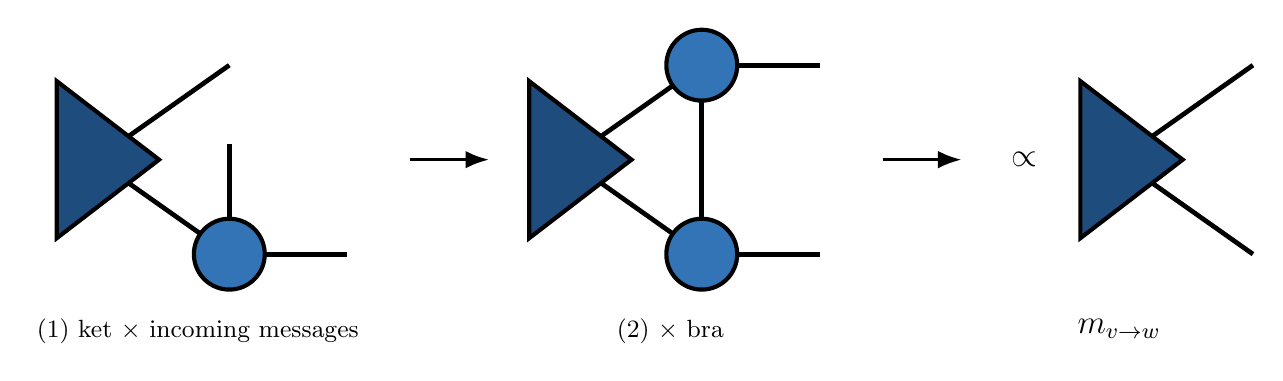
\begin{tikzpicture}
  % (1) ket with the incoming message absorbed; the bra leg of the message is still free
  \begin{scope}
    \coordinate (M) at (0,1.2);
    \coordinate (k) at (1.7,0);
    \draw[leg] (M) -- (k);
    \draw[leg] (M) -- (1.7,2.4);
    \draw[leg] (k) -- ++(0,1.4);
    \draw[leg] (k) -- ++(1.5,0);
    \node[msgmat] at (M) {};
    \node[tensor] at (k) {};
    \node[anchor=north,align=center] at (1.3,-0.7) {\small(1) ket $\times$ incoming messages};
  \end{scope}
  \draw[arrow] (4.0,1.2) -- (5.0,1.2);
  % (2) close with the bra
  \begin{scope}[xshift=6.0cm]
    \coordinate (M) at (0,1.2);
    \coordinate (k) at (1.7,0); \coordinate (b) at (1.7,2.4);
    \draw[leg] (M) -- (k); \draw[leg] (M) -- (b);
    \draw[leg] (k) -- (b);
    \draw[leg] (k) -- ++(1.5,0); \draw[leg] (b) -- ++(1.5,0);
    \node[msgmat] at (M) {};
    \node[tensor] at (k) {}; \node[tensor] at (b) {};
    \node[anchor=north,align=center] at (1.3,-0.7) {\small(2) $\times$ bra};
  \end{scope}
  \draw[arrow] (10.0,1.2) -- (11.0,1.2);
  % (3) the new message
  \begin{scope}[xshift=11.8cm]
    \node[lab] at (0,1.2) {$\propto$};
    \coordinate (N) at (1.2,1.2);
    \draw[leg] (N) -- (2.9,0); \draw[leg] (N) -- (2.9,2.4);
    \node[msgmat] at (N) {};
    \node[lab,anchor=north] at (1.2,-0.7) {$m_{v \to w}$};
  \end{scope}
\end{tikzpicture}
\end{document}
